The \dendro~ framework enables large-scale distributed memory computations on octree-refined adaptive meshes. Since the automatic code generation framework relies on \dendro ~for all distributed memory parallelization, we first present a high-level overview of \dendro.

\subsection{Distributed-memory parallelism}
%\mf{Quick overview of dendro. Focus mainly on zip/unzip and how the distributed problem is converted into a set of regular blocks, making it easy to use auto-generated codes.}
\dendro~ is a distributed memory adaptive octree based computational frameworks to solve the problem of compact binary object mergers. The problem of compact binary mergers can be mathematically represented by the BSSN/CCZ4 formulations of Einstien's field equations, and we use finite difference with the method of lines with Runge-Kutta (RK) time stepping to evolve the solution in time. Performing finite difference computations on an adaptive grid can be challenging due to the fact that spatial discretization $dx$ should be constant across the nodal dependance of the stencil.  
\par \dendro~ tackles this problem by the \zip~ \& \unzip~ representations of a distributed array. The key idea behind the \zip~ \& \unzip~ representations is that any arbitrarily adaptive octree can be decomposed into a set of regular sub-octrees (we refer this process as octree to block decomposition).  In the process of \unzip~, each sub-octree (i.e. regular block) is padded with the required number of grid point layers in order to perform finite difference stencil operations (see Figure \ref{fig:unzip}). The \zip~ operation refers to the inverse process of the \unzip ~operation where it copies data from a \unzip~ representation to a \zip~ representation of an array. The \unzip~ representation of a zipped array (i.e. a distributed array) is local to each process which means that there is no meaning to \unzip~ distributed array, hence the term distributed array always refers to the zipped representation. Note that all the interprocess communications happen in the \zip~ representation and \unzip representation is used only in locally to compute the derivative operations with the right-hand side of the equations to perform RK time stepping.   

\begin{figure}[tbh]
	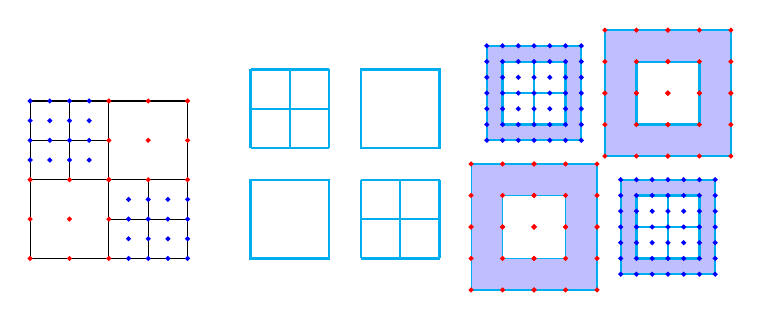
\begin{tikzpicture}[scale=0.2,every node/.style={scale=0.6}]
		
	\begin{scope}[shift={(0,0)}]
	\draw[step=5cm] (0,0) grid +(10,10);
	\draw[step=2.5cm] (5,0) grid +(5,5);
	\draw[step=2.5cm] (0,5) grid +(5,5);
	
	\def \r{0.12}
	\foreach \x in {0,2.5,5}{
	\foreach \y in {0,2.5,5}{
		\draw[red,fill=red] (\x,\y) circle (\r);
      }
	}
	
	\foreach \x in {5,7.5,10}{
	\foreach \y in {5,7.5,10}{
		\draw[red,fill=red] (\x,\y) circle (\r);
      }
	}

	\foreach \x in {0,1.25,2.5,3.75}{
	\foreach \y in {6.25,7.5,8.75,10}{
		\draw[blue,fill=blue] (\x,\y) circle (\r);
      }
	}	
	
	\foreach \x in {6.25,7.5,8.75,10}{
	\foreach \y in {0,1.25,2.5,3.75}{
		\draw[blue,fill=blue] (\x,\y) circle (\r);
      }
	}
	\end{scope}
	
	\begin{scope}[shift={(14,0)}]
	%\draw[cyan,thick,fill=blue!20] (-1,-1) rectangle +(6,6);
	\draw[cyan,thick] (0,0) rectangle +(5,5);
	\draw[cyan,thick,xshift=2cm,yshift=2.0cm] (5,5) rectangle +(5,5);
	\draw[cyan,thick,step=2.5cm,xshift=2.0cm] (5,0) grid +(5,5);
	\draw[cyan,thick,step=2.5cm,yshift=2.0cm] (0,5) grid +(5,5);
%	\draw[cyan,thick] (0,4) rectangle +(2,2);
%	\draw[cyan,thick] (2,4) rectangle +(2,2);
%	\draw[cyan,thick] (2,6) rectangle +(2,2);
%	\draw[cyan,thick] (4,0) rectangle +(2,2);
%	\draw[cyan,thick] (6,2) rectangle +(2,2);
%	\draw[cyan,thick] (6,0) rectangle +(2,2);
	\end{scope}
	
	\begin{scope}[shift={(30,0)}]
	\def \r{0.12}
	\draw[cyan,fill=blue!50,fill opacity=0.5]
	(-2,-2)--(-2,6)--(6,6)--(6,-2)--cycle
	(0,0) -- (4,0)-- (4,4)--(0,4)--cycle;
	\foreach \x in {-2,0,2,2,4,6}{
	\foreach \y in {-2,0,2,2,4,6}{
		\draw[red,fill=red] (\x,\y) circle (\r);
      }
	}
	
	\draw[cyan,thick,fill=blue!50,fill opacity=0.5,even odd rule,xshift=8.5cm,yshift=8.5cm] 
	(-2,-2)--(-2,6)--(6,6)--(6,-2)--cycle
	(0,0) -- (4,0)-- (4,4)--(0,4)--cycle;
		\foreach \x in {-2,0,2,2,4,6}{
	\foreach \y in {-2,0,2,2,4,6}{
		\draw[red,fill=red,xshift=8.5cm,yshift=8.5cm] (\x,\y) circle (\r);
      }
	}

	\draw[cyan,thick,fill=blue!50,fill opacity=0.5,even odd rule,xshift=8.5cm] 
	(-1,-1)--(-1,5)--(5,5)--(5,-1)--cycle
	(0,0) -- (4,0)-- (4,4)--(0,4)--cycle;
	\draw[cyan,thick,step=2,xshift=8.5cm] (0,0) grid +(4,4);
	\foreach \x in {-1,0,1,2,3,4,5}{
	\foreach \y in {-1,0,1,2,3,4,5}{
		\draw[blue,fill=blue,xshift=8.5cm] (\x,\y) circle (\r);
      }
	}
	
	\draw[cyan,thick,fill=blue!50,fill opacity=0.5,even odd rule,yshift=8.5cm] 
	(-1,-1)--(-1,5)--(5,5)--(5,-1)--cycle
	(0,0) -- (4,0)-- (4,4)--(0,4)--cycle;
	\draw[cyan,thick,step=2,yshift=8.5cm] (0,0) grid +(4,4);	
	\foreach \x in {-1,0,1,2,3,4,5}{
	\foreach \y in {-1,0,1,2,3,4,5}{
		\draw[blue,fill=blue,yshift=8.5cm] (\x,\y) circle (\r);
      }
	}
	
	\end{scope}	
	
	\end{tikzpicture}
	
\caption{\label{fig:unzip} \small A simplistic example of octree to block decomposition and \unzip~ operation. The leftmost figure shows the considering adaptive octree with \cgn~ and its block decomposition is shown in the middle. Note that the given octree is decomposed into four regular blocks of different sizes. The rightmost figure shows the decomposed blocks padded with values coming from neighboring octants with interpolation if needed.% In order to perform \unzip~ operation both $\psi$ and $\psi$ mappings are used. 
}
\vspace{-0.15in}
\end{figure}

\subsection{Symbolic interface for code generation}
\label{sec:symbolic}

Computational relativity simulations are usually governed by  non-linear, coupled, partial differential equations in curved spacetime. On discretization, one can end up with tens of equations with thousands of terms. 
Writing, optimizing and maintaining 
code for this is very challenging. Sustainability and keeping it relevant for new 
architectural changes are additional difficulties. To address these issues, we 
have developed a symbolic interface for computational relativity. We leverage symbolic python 
(\texttt{SymPy}) as the backend for this along with the python package 
\texttt{cog} to embed python code within our application-level \texttt{C++} 
code. The symbolic interface allows us to write the discretized 
versions of the equations similar to how they are written mathematically 
and enable improved usability for non-computational scientists. 

An example 
for the \BSSN~equations are shown in Figure \ref{fig:symb}, with the 
equations on the left and the corresponding python code on the right. 
%\mf{add figure}

\begin{figure*}[tbh]
	\noindent\fbox{
	\begin{minipage}[t]{.4\textwidth}
			\small
			\begin{eqnarray*}
			\partial_t \alpha &=&  \mathcal{L}_\beta\alpha - 2 \alpha K, \\
			\partial_t \beta^i &=& \lambda_2 \beta^j\,\partial_j\beta^i + \frac{3}{4} f(\alpha) B^i\\
			\partial_t B^i  &=& \partial_t \tilde\Gamma^i  - \eta B^{i}   + \lambda_3 \beta^j\,\partial_j B^i -\lambda_4 \beta^j\,\partial_j \tilde\Gamma^i \\
			\partial_t \tilde \gamma_{ij} &=&  \mathcal{L}_\beta\tilde{\gamma}_{ij} -2 \alpha \tilde A_{ij}, \\
			\partial_t \chi &=& \mathcal{L}_\beta\chi + \frac{2}{3}\chi \left(\alpha K -  
			\partial_a \beta^a\right)\\
			\partial_t \tilde A_{ij} &=& \mathcal{L}_\beta\tilde{A}_{ij} + \chi \left(-D_i D_j \alpha +
			\alpha R_{ij}\right)^{TF} +\nonumber \\
			&\,&\alpha \left(K \tilde A_{ij} -
			2 \tilde A_{ik} \tilde A^{k}_{\,j}\right), \label{eq:at_evol}\\
			\partial_t K &=& \beta^k\partial_kK- D^i D_i \alpha + \\
			&\,&\alpha \left(\tilde A_{ij}\tilde
			A^{ij} +\frac{1}{3}K^2\right),\\
			\partial_t \tilde \Gamma^i &=& \tilde \gamma^{jk} \partial_j
			\partial_k \beta^i + \frac{1}{3} \tilde \gamma^{ij} \partial_j
			\partial_k \beta^k + \beta^j \partial_j \tilde \Gamma^i - \nonumber \\
			&\,&\tilde
			\Gamma^j \partial_j \beta^i + 
			\frac{2}{3}\tilde \Gamma^i \partial_j
			\beta^j - 2 \tilde A^{i j}\partial_j \alpha + \nonumber \\
			&\,& 2 \alpha \left(\tilde
			{\Gamma^i}_{jk} \tilde A^{jk} + 6 \tilde A^{ij}\partial_j \phi -
			\frac{2}{3} \tilde \gamma^{ij} \partial_j K\right) \\
		 % ~ &~ & ~\\
			\end{eqnarray*}
	\end{minipage}% This must go next to `\end{minipage}`
	}
	\begin{minipage}[t]{.52\textwidth}
			\small
			\begin{minted}[frame=single,framesep=1pt]{python}
	
from OT_sym import *
	
a_rhs = OT.Lie(b, a) - 2*a*K
	
b_rhs = [3/4 * f(a) * B[i] + 
 	l2*vec_j_del_j(b, b[i]) for i in e_i]
	
B_rhs = [Gt_rhs[i] - eta * B[i] + 
	l3 * vec_j_del_j(b, B[i]) - 
	l4 * vec_j_del_j(b, Gt[i]) 
	for i in e_i]
	
gt_rhs =  OT.Lie(b, gt) - 2*a*At
	
chi_rhs = OT.Lie(b, chi) + 
	  2/3*chi*(a*K - del_j(b)) 
	
At_rhs = OT.Lie(b, At) + chi *
	 OT.TF(-DiDj(a) + a*OT.Ricci) +
	 a*(K*At -2*At_ikAtKj)
	
K_rhs = vec_k_del_k(K) - DIDi(a) +
	a*(1/3*K*K + A_ij_A_IJ(At)) 

	\end{minted}
	\end{minipage}
	\caption{\label{fig:symb} \small The left panel shows the \BSSN ~formulation of the 
	Einstein equations. These are tensor equations, with indices $i,j,\ldots$
	taking the values $1, 2, 3$. On the right we show the \texttt{{\dendro\_sym}}
	code for these equations. \texttt{\dendro\_sym} uses \texttt{SymPy} and other tools
	to generate optimized C++ code to evaluate the equations. Note that $\mathcal{L}_\beta,\ D,\ \partial$ denote Lie derivative, covariant derivative and partial derivative respectively, and we have excluded $\partial_t\Gamma^i$ from \texttt{\dendro\_sym} to save space. (See \cite{Baumgarte:1998te,Alcubierre:1138167} for more information about the equations and the differential operators.)}
	\label{fig:bssneqs}
	\vspace{-0.15in}
\end{figure*}

There are several
advantages to using a symbolic interface %like \texttt{\dendro\_sym}
for the application-specific equations. First, it greatly
improves the sustainability of the code by separating the 
high-level description of the equations from the low-level optimizations,
which can be handled by
architecture-specific code generators, such as \texttt{C++}, CUDA, etc. 
%We currently support \texttt{avx2} code-generators and \texttt{CUDA} generators--the focus of this work. 
Since these are applied at a
block level, it is straightforward to schedule these blocks across
cores or GPUs. Note that the auto-generated code consists of several
derivative terms that are spatially dependent as well as other point-wise
update operations. We use a hybrid approach to achieve both portability as well as high performance. We focus on developing auto generation methods for the pointwise operations, allowing high-level optimizations to be easily applied at the block level and combine with a library of specialized implementations based on the stencil-structure for the derivative terms. 

We leverage the code generation capabilities of SymPy, such as common subexpression elimination (CSE) \cite{cse} to 
minimize the number of operations. SymPy already supports naive \texttt{C++} code generation, so this is used as our baseline implementation. In the following sections, we highlight the characteristics of the naive \texttt{C++} code, and to the design of optimizations for the pointwise as well as the stencil operations.


%% Commenting for now - Hari - Can add later if needed.
% Different architectures such as GPUs, Multi-core CPUs and many core processors have different architectural capabilities that can be used to maximize the performance of DENDRO execution using parallelism. DENDRO execution for large data-blocks consumes large amount of memory. DENDRO code for computer systems which have less memory capacity, must be specifically configured for the execution of large data-blocks. Initial implementation of DENDRO library was not optimized for GPU. This paper focuses on approaches and research carried out to generate optimized GPU compatible code to execute corresponding computational process.
% \\
% Initial research is focused on converting sequential CPU execution logic of DENDRO to GPU compatible code using CUDA to exploit GPU parallelism. Block and thread allocation in GPU and sequential CPU logic conversion is done without exploiting system specific restrictions such as memory limitations, GPU architecture specific limitations or number of GPUs in a particular system. This stage of research considers only one GPU for the optimization. Memory restriction is ignored by limiting the block size of experiment. This stage primarily focuses on converting the sequential CPU logic of DENDRO to GPU and verifying the output of corresponding GPU code against the output of sequential CPU code to the same input data set.
% \\
% Following stages primarily focus on optimizing the CUDA code for GPU. These stages also assume that execution will be done on a single GPU system with enough memory. Vendor specific constraints for a given GPU is ignored. Optimization research is done to minimize time taken for data copying from host to device and device to host, minimize frequency of the memory allocations in the GPU, optimize cache usage and parallelize kernel execution in GPU. Each stage is tested against the output of serial execution of DENDRO for multiple levels of data blocks. Then, memory limitation and vendor specific restrictions for a given GPU are taken into consideration. Dynamic thread and block scheduling has also been introduced to the GPU code subsequently. Required memory for execution is also re-factored and restructured in order to be compatible with the memory restrictions of a given GPU. Above optimization changes are automatically generated based on globally setup parameters. Under above mentioned conditions, implemented GPU compatible version of DENDRO is tested on several GPU computer systems and speed up is recorded against CPU based serial execution.
% \\
% DENDRO optimization for multiple GPU based computer systems will not be covered by this paper.

\subsection{SymPy based GPU code generation}
\label{sec:naive}
%\mf{Can you refine this section.}
In this section, we discuss GPU code generation for SymPy based \BSSN~ symbolic equations (see Figure \ref{fig:symb}). \dendro~ octree to block decomposition makes the problem embarrassingly parallel which makes it easier to generate GPU code since there is no data dependencies between the octree blocks. The main task of the generated code would be to evaluate the \BSSN equations for each octree block using specified GPU architecture efficiently. In order to compute the right-hand side (RHS) of the BSSN equations, we need to apply finite difference approximations of derivative operators followed by the RHS computation. Note that \sympygr~ framework supports derivative computations in curved spacetime with respect to the specified coordinate system. The Lie ($\mathcal{L}_\beta$) and covariant ($D_i$) derivatives are computed based on the basis induced by the specified coordinate system hence converted into a collection of spatial derivatives. All the spatial derivative operators (i.e. $\partial_i ,\partial_{ij}$ for $i,j={1,2,3}$) are human written GPU derivative kernels, but the core RHS computation and call for the derivative kernels are machine generated by \sympygr~ framework.

%This stage primarily focuses on converting serial DENDRO logic to GPU based parallelized code using CUDA and verifying the generated output against output of the CPU version. DENDRO serial logic has no dependencies between the processing of two data-blocks. However for a given data-block, there is a certain sequentiality that must be followed and maintained when the data is processing. 
%DENDRO logic can be separated to 2 parts; derivative calculation and RHS calculation. 
%Derivative calculations have several methods for partial differential calculation on various directions. Each of these methods are treated as separate kernel calls in GPU as there is a specific order to be invoked, since required derivatives to be calculated may vary with the experiment. Furthermore, there can be dependencies introduced between each derivative calculation according to the experiment. RHS calculation logic calculate values per each array index. RHS calculation logic is a generated sequence of equations which is being optimized by another research carried on.

\begin{algorithm}
	\caption{\small \computeRHS: Overview of GPU based \BSSN evaluation}\label{alg:overview_gpu}
	\footnotesize
	\begin{algorithmic}[1]
		\Require A list of \zip~ variables $U_{zip}[]$, List of octree blocks $B$
		\Ensure  A list of \zip~ variables $V_{zip}[] \rightarrow \BSSN(U_{zip})$ \BSSN~ equations evaluated at
		\State $U_{unzip}[] \leftarrow unzipVars(U_{zip}[])$
		\State $\_U_{unzip}[] \leftarrow cudaMalloc(\text{sizeof}(U_{unzip}[]))$
        \State $\_V_{unzip}[] \leftarrow cudaMalloc(\text{sizeof}(V_{unzip}[]))$
        \State $cudaMemCopy(U_{unzip}[],\_U_{unzip}[],D2H)$	
        \For {$b \in B$}
        	\State $\_deriv[] \leftarrow allocateDerivs()$
            \State $\_deriv[] \leftarrow launchDerivKernals()$ 
            \State $\_V_{unzip}[] \leftarrow launchRHSKernal()$
        \EndFor
        \State $cudaMemCopy(V_{unzip}[],\_V_{unzip}[],H2D)$	
        \State $V_{zip}[] \leftarrow zipVars(V_{unzip}[])$
	\end{algorithmic}
\end{algorithm}

The basic approach for the GPU based \BSSN~ computation would be to process each octree block sequentially with GPU loop parallelism where each grid point in a given octree block is computed parallel threads. In this approach, data communications between the CPU \&  the GPU performed in a synchronous manner using blocking communication calls. In the basic implementation, data for all the octree blocks are transferred to the GPU as a single 1D array. When a octree block is processed, the data for that specific octree block is identified using an \textit{offset} value that is passed for every kernel execution. Subsequently, a single output array is used to get the output of the processed octree blocks. \sympygr~ uses the common sub-expression elimination approach in the SymPy framework to eliminate repetitive computations by storing them in temporary variables which are thread local while octree block derivative \& input variables are GPU block local. Even though the basic code generation for the core RHS computation is fairly trivial, we can use additional GPU level optimizations to perform GPU computations efficiently.



%In the serial CPU version, values are calculated for indexes of 3D array which are effectively converted to loop parallelism in the GPU code. Kernel calls are fully synchronized and no optimization tasks are carried out. Each data-block is treated as a separate operation which is being executed one after the other. In order to execute the process for one block, intermediate data arrays have to be allocated in the GPU before the execution of each block. Those required memory allocations for derivative operations and RHS operation were done separately for each data-block. These allocations are released in GPU after the processing of each data-block. However two global arrays are used in the GPU to store data required for all the blocks and to store the output generated by the processing of all the data-blocks. Offsets are given per data-block process to determine which part of the input and output arrays should be accessed in each processing of a data-block. After processing all the data-blocks, output array is copied back to host from the GPU. Then, memory allocations for input and output arrays are released in GPU. Copied version of output to host is tested against the serial DENDRO output in order to verify the correctness of the GPU compatible code. Additionally this test confirms the convertibility of DENDRO serial logic to GPU based parallelized logic.
%Figure \ref{fig:whole_process} shows GPU profiling details for the implementation of step 1 using input of 5 data-blocks of block level 4.

%While it is fairly straightforward to generate CUDA (or other) code from SymPY expressions, it is far more challenging to get good performance for such code. In the following sections, we highlight the optimizations we performed to ensure that the performance of the auto-generated code is comparable to hand optimized code. 
% Note, that while these optimizations were done by careful profiling and parametrization of the generated code, these work in conjunction with the code generation framework and will also benefit 
% This is put in the algo. pseudo code. 
% \begin{figure}
%    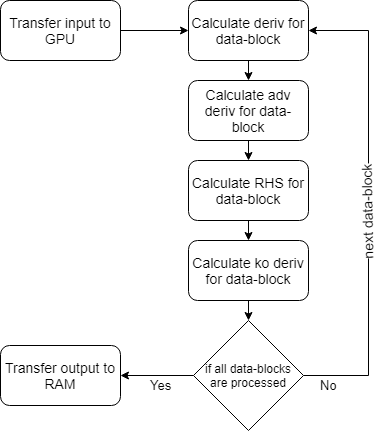
\includegraphics[width=\linewidth]{./images/flow.png}
%   \caption{Flow of Process}
%   \label{fig:flow}
% \end{figure}

\begin{figure}
  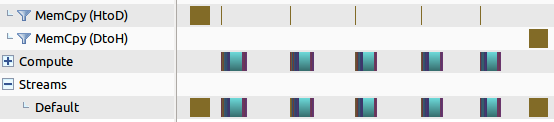
\includegraphics[width=\linewidth]{./images/basic.png}
  \caption{GPU profiling of step 1}
  \label{fig:whole_process}
\end{figure}

\begin{figure}
  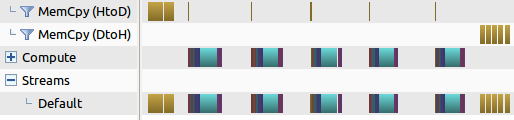
\includegraphics[width=\linewidth]{./images/structure_change.png}
  \caption{GPU profiling of step 2}
  \label{fig:structure_change}
\end{figure}

\subsection{Restructuring the input for better cache optimization}
\label{sec:cache}
When a given octree block is computed, specific partition (i.e. based on the octree block offset) of the input and output octree block global data arrays needs to be accessed. This access pattern can be lead to false-sharing when we perform multiple octree blocks at a single instant. Note that the access locations for each octree block is unique and does not overlap with other octree blocks (due to the \unzip~ representation). In order to minimize the cache misses during the octree block computations we can restructure the input \& output arrays corresponding to the octree block being processed. In this approach, instead of global input/output arrays, we create octree block local input/output arrays which are bundled together and data is copied from global to local arrays prior to the kernel launch. 

%Additionally, when a block is processed, the data has to be accessed from specific memory locations of the 1D array but not from consecutive memory locations. Furthermore, those memory locations are not accessed for processing of other blocks as well. Output is also written to the independent memory locations of the output array but not to the consecutive memory locations. When the execution is carried out for a block, there have been too much cache misses since the data to be accessed is in diverse memory locations. When the output is written back to the memory, cache misses occurs once again because output is also written to diversified memory locations. Since the input and output data for one block is independent from other blocks, by simply changing the structure of the input and the output, it is possible to gain much cache performance. In this approach, instead of creating a large 1D input array, required data for the execution of one block is taken to consecutive memory locations and bundle together. Then the data is copied from host to device before the start of kernels and copied back to the main memory after the execution is finished. As in the Step 1, required temporary memory allocations for derivative operations were done separately for each data-block. These allocations were also released subsequently in GPU after the processing of each data-block. Since in this approach all the data is in consecutive memory locations, it was possible to gain a remarkable speedup through the cache optimization.

\subsection{Minimizing Reallocations}
\label{sec:allocs}
The number of derivative computations required to compute the \BSSN~ equations is a constant across the input octree blocks but size of the allocation depends on the number of grid points in the octree block which can vary across the blocks. These derivative allocations are local to each octree block which are used to store the output of derivative kernels. Performing memory allocations/de-allocations for each octree block can be avoided by using the upper bound of the number of grid points across all the blocks. Hence we can perform a single memory allocation for derivative computations which can accommodate any given octree block in the input block list. 

%In the \S\ref{sec:cache}, it had overhead of memory re-allocation for temporary arrays which are used to store the output of derivative functions. These allocations required to be released at the end of each data-block iteration which introduced even more overhead. Even though the number of temporary arrays required are same for each data-block, size of each temporary array depends on the level of the data-block. Hence, before the execution of any data-block in GPU, memory allocations for temporary arrays are done such that they can occupy the data which needs to process the largest data-block in the input data-block set. In this approach, these temporary arrays can be used to process all the data-blocks given without re-allocating repeatedly. All memory allocations are released at the end whole process.

\begin{figure}
  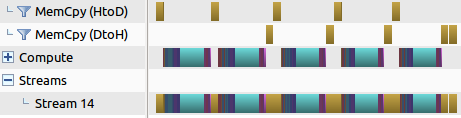
\includegraphics[width=\linewidth]{./images/no_realloc.png}
  \caption{GPU profiling of step 3}
  \label{fig:no_realloc}
\end{figure}

\subsection{Block-wise asynchronous data transfers}
\label{sec:async}
In order to improve the performance of data transfer between the host and the device, we use asynchronous octree block-wise data transfers. Initially, the first iteration of octree block data transfer is synchronous, but the consequent blocks can be transferred to the device, while the previous octree blocks being processed by the GPU. Similarly, we can use asynchronous data transfers to copy the computed output from the device to the host.

%Previous steps show considerable overhead in data copy from host to device and device to host.  This step is an extension of \S\ref{sec:allocs} to minimize overhead of data transfer. First iteration of data-block must be synchronized with data transfer of its input array. But input array for other data-blocks can be transfered to device while the kernel process happens for previous data-block. Output of each iteration can be transfered to host while kernels of the next iteration is being executed. But, the process must ensure none of the kernels of any data-block iteration starts before its input array is fully transfered to device. Hence proper synchronization between data transfer and processing should be maintained. Figure \ref{fig:kernal_memcpy_overlap} shows GPU profiling for this configuration.

\begin{figure}
  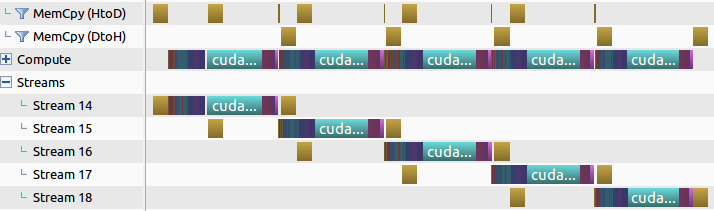
\includegraphics[width=\linewidth]{./images/kernal_memcpy_overlap.png}
  \caption{GPU profiling of step 4}
  \label{fig:kernal_memcpy_overlap}
\end{figure}

\subsection{Overlapping the device and the host communications}
\label{sec:overlap}
The block-wise asynchronous data transfers can perform the transfers in a non-blocking fashion, we can further improve the performance of the data movement between the host and the device by enabling simultaneous data movement from the host to the device and vice versa. Simultaneous two-way data transfers need specific hardware support and can be only achieved by the GPU architectures which have duel memory copy engines. 

% How is the below passage is relevant in this section. - Milinda 
% It take more time because of the altering of memory allocation method. i used it to justify the performance reduce.This is the only change introduced from previous iteration  - Eminda
\par Based on how CUDA compiler memory layout, the host memory is categorized as pageable and pinned memory. The pageable memory is used as default memory allocation unless specified otherwise. The device cannot directly access the pageable host memory hence when a data transfer is evoked between the host and the device, the device will allocate temporary pinned memory and the host will copy data from pageable memory to pinned memory prior to the actual data transfer begins.  

%there are mainly two types of host memory. One is pageable memory and the other one is pinned memory which prevents memory from being swapped out. Pageable memory is used as default memory allocation in host unless it is specifically defined. The GPU cannot access data directly from pageable host memory, so when data transfer from pageable host memory to device memory is invoked, the CUDA driver must first allocate a temporary pinned memory, copy the host data to the pinned memory, and then transfer the data from the pinned memory to device memory. In order to make host to device and device to host memory to be overlapped, all the data transfers should use only pinned memory.

%Although introducing block-wise asynchronous data transfers approach  has asynchronous data transfer capabilities, it was not possible to transfer data from HtoD and DtoH at the same time. Therefore, data transfer can be further improved by achieving HtoD and DtoH overlap. This type of parallelism can only be achieved by GPUs with duel memcopy engines. However this implementation was carried out to compare pros and cons of parallelizing data transfers between host and device. There are two type of host memories. One is pageable memory and the other one is pinned memory which prevents memory from being swapped out. Pageable memory is used as default memory allocation in host unless it is specifically defined. The GPU cannot access data directly from pageable host memory, so when data transfer from pageable host memory to device memory is invoked, the CUDA driver must first allocate a temporary pinned memory, copy the host data to the pinned memory, and then transfer the data from the pinned memory to device memory. In order to make host to device and device to host memory to be overlapped, all the data transfers should use only pinned memory.
\begin{figure}
  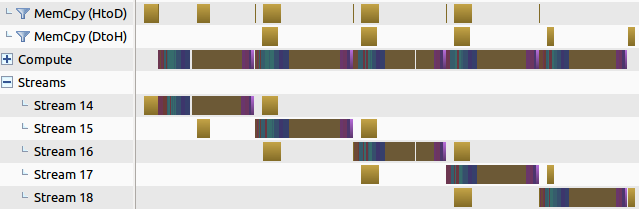
\includegraphics[width=\linewidth]{./images/duel_mem_cpy.png}
  \caption{GPU profiling of step 5}
  \label{fig:duel_mem_cpy}
\end{figure}
Figure \ref{fig:duel_mem_cpy} shows profiling of step 6 parallel data transfer implementation.
%New section -Eminda -please change if wants to
\subsection{Thread load optimization and data-block process parallelization}
\begin{figure}
  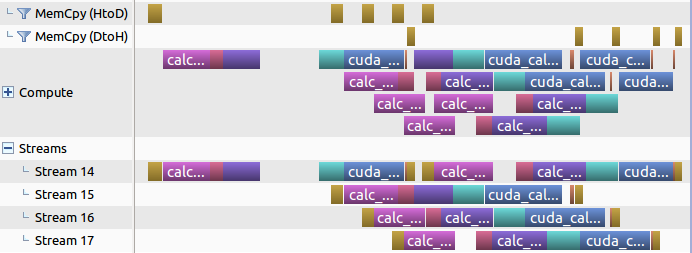
\includegraphics[width=\linewidth]{./images/4streams.png}
  \caption{GPU profiling of step 7}
  \label{fig:four_streams}
\end{figure}
Previous steps had too many kernal calls yet too little computation for each kernal since kernals were created for each different logical computation. In the first step of this iteration all deriv operation types were brought forward to one single kernal. Dynamic configuration for deriv methods were taken place inside kernal call itself. In the second stage, deriv kernal and rhs kernal were reconfigured to allocate more than one memory point in octal tree increasing load of GPU thread. This process can be used to effectively free portion of GPU for other streams for small level data-block processing enabling parallelism between multiple data-blocks.
\ref{fig:four_streams} shows profiling of this iteration when 4 streams are used for 0 level 4 data-block with optimal load balancing for each GPU thread.

\subsection{Architecture specific Optimizations}
\label{sec:arch}

% I guess we should clearly mention how the octree block scheduling is automated across different GPU architectures. Need to mention clearly available set of parameters and how those parameters can be changed to achieve good performance for a given architecture. - Milinda'
%
% These are the current available parameterizations
% threads_per_block 1024
% threads_per_block_rhs 250 - can tune to achieve best of registers. 
% thread_load_deriv 5 - number of collective data points handled by a single thread
% thread_load_adv_deriv 5 - number of collective data points handled by a single thread
% thread_load_rhs 1 - number of collective data points handled by a single thread
% thread_load_ko_deriv 5 - number of collective data points handled by a single thread
% thread_load_output 1 - number of collective data points handled by a single thread
%
% thread load can be increased to increase the work load of a single thread. By increasing this we can free part of GPU for another data block process. This is good for increase of throughput. But highly depend on GPU. It is bit hard to find the best tuning point. Very good if lot of small blocks.
% numberOfStreams 4 - number of parallel executable data blocks
% GPUCapacity 6000 - memory capacity

Previous steps didn't consider vendor specific limitations for development or optimization. Different GPUs have different memory capacities. Both total memory capacity of GPU and number of total registers available per block affect execution of \dendro. Moreover, different GPU architectures perform differently to the same CUDA implementation. For a better optimization \dendro needs to switch for the best implementation approach for a given GPU. Some GPUs does not have duel memcopy engines, in which overlapping of the host and the device communications will not happen. Hence step 5 was parameterized to create pinned memory only if the specific GPU has duel memcopy engines. Execution of step 5 in a GPU without duel memcopy engines results in the same profiling of step 4 but with less efficiency because of time consumed to pinned memory allocation. Considering these limitations to achieve best performance, \dendro CUDA implementation should be parameterized so that implementation can be altered according to the GPU which is used.
\\Step 1 and 2 do not work for GPUs with less memory when multiple data-blocks of higher levels are executed, even though they can cater for execution each data-block separately. But in the step 3, 4 and 5, there is a parameter to specify the capacity of the GPU. Based on that value data-blocks are scheduled to be processed without exceeding the memory.
\\RHS kernel execution require huge number of variable initialization inside each thread. Each block of GPU has certain number of registers. When total number of variable initialization inside block can not fit for total number of registers available, execution process halts with errors. This problem can be solved by limiting the number of effective threads per block used for RHS calculation. This limitation can be optimized for a specific GPU considering the number of registers available per block in vendor specification. This can be achieved by parameterizing the number of threads per block in RHS operation.
\\ %Below paragraph is a new entry- Eminda - Please check and change, if wants to
GPU threads have different capacity for the amount of work required to efficiently execute based on specific GPU. Asynchronous data transfer step was parameterized to execute deriv and rhs operation for multiple points defined by a single GPU thread. Operating multiple points by a single GPU frees portion of GPU which can be used to process another data block. For a better optimization load per thread should be balanced to optimal GPU sharing between 2 ore more data blocks.
\\These parameters can be either manually set or automatically set via a program that checks specific GPU limitations chosen for the execution. Configuration and optimization for multiple GPU systems remains for experiment.
